\documentclass[border=3pt,varwidth]{standalone}
\usepackage{amsmath,amssymb}
\usepackage{tikz}
\usetikzlibrary{arrows.meta,calc,decorations.markings,patterns,positioning,angles,quotes}
\tikzset{
  >=Stealth,
  every node/.style={font=\normalsize},
  wire/.style={line width=0.9pt},
  thinwire/.style={line width=0.6pt},
  fieldline/.style={line width=0.6pt,-{Stealth[length=2.2mm]}},
  axis/.style={line width=0.7pt,-{Stealth[length=2.2mm]}},
  dashedwire/.style={line width=0.9pt,dash pattern=on 3pt off 2pt},
  resistor/.style={line width=0.9pt},
  chargepos/.style={circle,draw,line width=0.8pt,minimum size=5mm,inner sep=0pt},
  dotcharge/.style={circle,fill,inner sep=0pt,minimum size=2.4pt}
}
% Draw a resistor box centered at (x,y) with width w, height h, horizontal
\newcommand{\resbox}[4]{%
  % #1=x #2=y #3=halfwidth #4=label
  \draw[resistor] (#1-#3,#2-0.18) rectangle (#1+#3,#2+0.18);
  \ifx\\#4\\\else\node[above=2pt] at (#1,#2+0.18) {#4};\fi
}
% Battery symbol: long thin line (+) then short thick line (-), centered at (x,y)
\newcommand{\battery}[2]{%
  % #1=x #2=y ; long line left=+, short line right=- by default orientation
  \draw[wire] (#1-0.09,#2-0.32) -- (#1-0.09,#2+0.32);
  \draw[line width=2.6pt] (#1+0.09,#2-0.16) -- (#1+0.09,#2+0.16);
}

\begin{document}
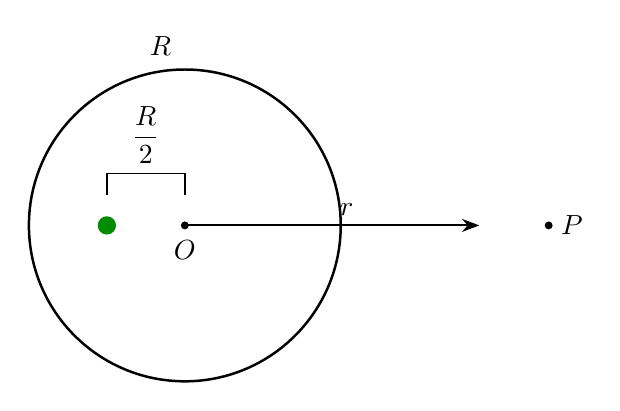
\begin{tikzpicture}[scale=1.1]
  \def\R{1.8}
  \draw[wire] (0,0) circle (\R);
  \fill (0,0) circle (1.3pt);
  \node[below=2pt] at (0,0) {$O$};
  % point charge at R/2 to the left of O
  \coordinate (q) at (-0.9,0);
  \fill[green!55!black] (q) circle (3pt);
  % bracket showing R/2 from charge to O
  \draw[thinwire] (q) ++(0,0.35) -- ++(0,0.25) -- (0,0.6) -- ++(0,-0.25);
  \node[above] at (-0.45,0.6) {$\dfrac{R}{2}$};
  \node[above left=2pt] at (0,\R) {$R$};
  % axis from O to P outside
  \draw[axis] (0,0) -- (3.4,0) node[pos=0.55,above]{$r$};
  \coordinate (P) at (4.2,0);
  \fill (P) circle (1.3pt);
  \node[right=1pt] at (P) {$P$};
\end{tikzpicture}
\end{document}
